%%%%%%%%%%%%%%%%%%%%%%%%%%%%%%%%%%%%%%%%%%%%%%%%%%%
%% Environnement et outils
%%%%%%%%%%%%%%%%%%%%%%%%%%%%%%%%%%%%%%%%%%%%%%%%%%%
\section{Environnements et outils}
\addcontentsline{toc}{subsection}{Introduction}
\subsection*{Introduction}

Après avoir présenté les différentes étapes de conception et la méthodologie suivie, nous présenterons dans ce chapitre les outils de développement et les différents composants logiciels et matériels, pour lesquels constituent la mise en œuvre effective des différentes tâches du sujet.

\subsection{Composants logiciels}
\subsubsection{Front-end}
\begin{longtblr}[caption={Technologies utilisées au niveau du front-end}]{
    hlines = {0.25pt,cyan6},
    vlines = {0.25pt,cyan6},
    row{odd} = {bg=cyan9!10!white},
    colsep=4pt,
    rowsep=4pt,
	colspec={cX},
    rowspec={Q[m] Q[m] Q[m] Q[m] Q[m] Q[m]},
}
{

\includegraphics[height=8mm]{images/sec5/bootstrap.pdf}
\\\textbf{Bootstrap}
}
& 
Bootstrap est un framework front-end extrêmement robuste permettant de développer des applications et des sites Web de manière plus rapide et plus conviviale. Il comprend des modèles de conception basés sur HTML et CSS pour les composants d'interface utilisateur courants tels que les formulaires, les boutons, les tableaux, les navigations, les alertes, les onglets et bien d'autres, ainsi que les extensions JavaScript optionnelles.
Bootstrap offre également la possibilité de créer des mises en page réactives (responsive design) avec un effort minimal.\\

{

\includegraphics[height=6mm]{images/sec5/elementui.pdf}\\\textbf{Element UI}
}
& 
Element est une bibliothèque de composants d'interface utilisateur basée sur Vue 2.0 et qui jouit du soutien d'une large communauté. Elle n'est pas seulement destinée aux développeurs front-end, mais fournit également un kit d'interface utilisateur complet avec lequel les concepteurs et les chefs de produit peuvent travailler. Elle est spécifiquement conçue pour la création d'interfaces utilisateur de bureau, mais prend en charge certaines fonctionnalités réactives telles que le masquage des éléments en fonction de la taille de la fenêtre et la création de grilles.
\\

{
\includegraphics[height=5.5mm]{images/sec5/jquery.pdf}
 \\\textbf{jQuery}
}
&  
\begin{minipage}{\linewidth}
jQuery est une bibliothèque JavaScript libre créée pour faciliter l'écriture de scripts côté client dans le code HTML des pages web. Elle propose comme principales fonctionnalités :
\raggedright
\begin{itemize}[leftmargin=*]
\item La manipulation du Document Object Model (DOM).
\item La gestion des événements (mouvements de souris, clics, etc.) et de l'AJAX.
\item La création d'effets d'animation.
\item La manipulation des feuilles de style en cascade.
\end{itemize}
\end{minipage}
\\
{
\includegraphics[height=5.5mm]{images/sec5/jqueryui.pdf}
 \\\textbf{jQuery UI}
 }
 & 
 \begin{minipage}{\linewidth}
	jQuery UI est une bibliothèque JavaScript basée sur jQuery, fournissant une collection d'éléments utiles au développement d'interfaces utilisateur. Ces éléments comprennent :
\begin{itemize}[leftmargin=*]
	\item Des interactions comme le "drag \& drop" (glisser-déposer)
	\item Des "widgets" (composants d'interface graphique) telles que les barres de progression, les infobulles, etc.
	\item Des effets pour modifier dynamiquement l'apparence des éléments de l'interface (par exemple, changer la couleur, faire apparaître/disparaître un élément, etc.)
	\item Des thèmes avec des propriétés CSS pour la mise en page des éléments interactifs.
\end{itemize}
\end{minipage}
 \\
 {
\includegraphics[height=8mm]{images/sec5/sass.pdf}
 \\\textbf{Sass}
 }
 & Sass (Syntactically Awesome Style Sheets) est une extension de CSS intégrant des fonctionnalités telles que les règles imbriquées, les variables, les mixins et les extensions de classe. Cela permet aux développeurs d'écrire des CSS structurés, lisibles et réutilisables. Sass est compilé en CSS standard. Il s'agit principalement d'un langage de préprocesseur CSS qui accepte à la fois le CSS et sa syntaxe personnalisée d'écriture de codes de conception visuelle.\\
{
\includegraphics[width=8mm]{images/vuejs.png} \\\textbf{VueJs}
} & Vue (prononcé /vju:/, comme le terme anglais view) est un framework évolutif pour construire des interfaces utilisateur. À la différence des autres frameworks monolithiques, Vue a été conçu et pensé pour pouvoir être adopté de manière incrémentale. Le cœur de la bibliothèque se concentre uniquement sur la partie front-end. D’un autre côté, Vue est tout à fait capable de faire tourner des applications web mono-pages quand il est couplé avec des outils modernes et des bibliothèques complémentaires.\\
\end{longtblr}

\subsubsection{Back-end}
\begin{longtblr}[caption={Technologies utilisées pour les solutions back-end}]{
    hlines = {0.25pt,azure6},
    vlines = {0.25pt,azure6},
    row{odd} = {bg=azure9!10!white},
    colsep=4pt,
    rowsep=4pt,
	colspec={cX},
    rowspec={Q[m] Q[m] Q[m] Q[m] Q[m] Q[m]},
}
{
\includegraphics[height=4.5mm]{images/sec5/hibernate.pdf}
 \\\textbf{Hibernate}
 }
 & Hibernate est une bibliothèque de mappage objet-relationnel (ORM) pour le langage Java permettant aux développeurs d'utiliser des modèles de domaine de style POJO dans leurs applications d'une manière qui va bien au-delà du mappage objet/relationnel.\\
 {
\includegraphics[width=7mm]{images/sec5/java.pdf}
 \\\textbf{Java}
 }
 & JAVA est un langage de programmation de haut niveau, orienté objet, fonctionnel, indépendant de la plate-forme et un environnement d'exécution.
 Le langage Java tire une grande partie de sa syntaxe du C et du C++, mais son modèle objet est plus simple que celui de ce dernier et il a moins de facilités de bas niveau. Les applications Java sont généralement compilées en bytecode (appelés fichiers de classe) qui peuvent être exécutés par une JVM (Java Virtual Machine), indépendamment de l'architecture informatique. La JVM compile souvent le code en code machine natif pour optimiser les performances.\\
{

\includegraphics[height=6.5mm]{images/sec5/log4j.png}
\\\textbf{Log4j}
}
& Log4j est un outil de journalisation permettant de personnaliser les logs propres à chaque programme. Il peut être utile pour le débogage ou le traçage de l'exécution d'un programme.\\
{

\includegraphics[height=5.5mm]{images/sec5/spring.pdf}
\\\textbf{Spring}
}
& 
Spring est un framework open source fournissant une boite à outils très riche permettant de structurer, d'améliorer et de simplifier l'écriture d'application Java. Spring est également livré avec une variété de modules dédiés à l'exécution de différentes tâches. Certains d'entre eux sont Spring Test, Spring Security, Spring Web, Spring JDBC, Spring AOP, Spring MVC et Spring ORM.\\

{

\includegraphics[height=5.5mm]{images/sec5/spring.pdf}\\\textbf{Spring Batch}
}
& 
Spring Batch est un framework open source basé sur Spring pour permettre le développement d'applications batch qui sont essentielles au fonctionnement quotidien des systèmes d'entreprise. En général, les applications batch font référence à des systèmes automatisés conçus pour traiter des données de masse.
Spring Batch automatise cette itération de base des lots, en offrant la possibilité de traiter des transactions similaires comme un ensemble, souvent dans un environnement isolé, sans aucune interaction avec l'utilisateur.
\\

 {
\includegraphics[height=5.5mm]{images/sec5/spring.pdf}
 \\\textbf{Spring Boot}
 }
&  
\begin{minipage}{\linewidth}
Spring Boot permet de créer facilement une application alimentée par Spring avec un minimum d'effort. Une application créée avec Spring Boot peut être :
\raggedright
\begin{itemize}[leftmargin=*]
\item Créée sans requérir aucune configuration xml.
\item Créé sans aucune exigence de serveur d'application puisque Spring Boot fournit un serveur d'application (Tomcat intégré, Jetty ou Undertow).
\item Largement configuré avec quelques valeurs par défaut et des POM de démarrage pour simplifier la configuration Maven du projet.
\item Fournit des solutions prêtes pour la production telles que les métriques, l'intégrité de performance et la configuration externalisée.
\end{itemize}
\end{minipage}
\end{longtblr}
\subsubsection{Système de gestion de base de données}
Arkevia est conçu pour fonctionner sur une instance Oracle 10g  (ou plus).\\
Le SGBDR \textbf{Oracle} est utilisé par toutes les applications de la solution ARKEVIA. Il dispose aujourd'hui de l'une des meilleures prestations en termes de performance, de scalabilité et d'administration.
\subsubsection{Stockage et sécurité des données}
Le coffre-fort électronique constitue un espace de stockage sécurisé pour les documents qui y sont déposés (EDI, EDI signé, PDF signé).\\
Il permet de garantir :
\begin{itemize}
    \item L'intégrité des documents, au moyen d’une fonction de signature électronique.
    \item La confidentialité des documents, au moyen d’une fonction de chiffrement de données.
    \item La traçabilité des actions effectuées (dépôts, restitutions, demandes de copies, etc.).
    \item Les documents ont ainsi une valeur probante(juridiquement opposable).\\
\end{itemize}
\begin{itemize}[leftmargin=*]
    \item[\textcolor{green5!30!white}{\faCheckCircleO}] Le dépôt ou l'extraction de fichiers ne peut se faire qu'à partir de l'application ARKEVIA, via les Web Services avec authentification SSL Client/Serveur.
    \item[\textcolor{green5!30!white}{\faCheckCircleO}] Les fichiers sont horodatés, signés, chiffrés et stockés dans un espace sécurisé du datacenter de Cegedim.\newpage
    \item[\textcolor{green5!30!white}{\faCheckCircleO}] Le contenu est chiffré avec l'algorithme AES 128 GCM, la clé appartient à Cegedim. Le chiffrement des flux est sécurisé en HTTPS / TLS 1.2 (AES 256) avec un certificat SHA-256 appartenant à Cegedim.
    \item[\textcolor{green5!30!white}{\faCheckCircleO}] Les mots de passe des utilisateurs sont protégés par « hashage » via l'algorithme SHA-256.
\end{itemize}
\subsection{Environnement de développement}
\subsubsection{Environment matériel}
Les tâches assignées ont été élaborées sur un ordinateur de bureau conçu pour réaliser les différentes activités liées aux thèmes du stage, soit directement, soit par le biais du protocole RDP. L'ordinateur fourni a les spécifications matérielles et logicielles suivantes :
\begin{itemize}
    \item \textbf{Fabricant} : Dell Inc.
    \item \textbf{Modèle du système} : OptiPlex 7040
    \item \textbf{Processeur} : [01] : Intel64 Family 6 Model 94 Stepping 3 GenuineIntel ~3312 MHz
    \item \textbf{Mémoire physique totale} :  16 309 Mo
    \item \textbf{Système d’exploitation} : Microsoft Windows 10 Professionnel pour les Stations de travail.
\end{itemize}

\subsubsection{Environnement logiciel et outils}
\begin{longtblr}[caption={Environnements et outils de développement et de collaboration}]{
    hlines = {0.25pt,red7},
    vlines = {0.25pt,red7},
    row{odd} = {bg=red9!10!white},
    colsep=4pt,
    rowsep=4pt,
	colspec={cX},
    rowspec={Q[m] Q[m] Q[m] Q[m] Q[m] Q[m] Q[m] Q[m] Q[m] Q[m] Q[m] Q[m] Q[m] Q[m] Q[m] Q[m] Q[m] Q[m]},
}
{

\includegraphics[height=8mm]{images/sec5/confluence.pdf}
\\\textbf{Confluence}
}
& 
Atlassian Confluence est un système de collaboration et de wiki pour les entreprises.
Atlassian Confluence est utilisé pour la collaboration, la gestion de la base de connaissances, la rédaction technique et en tant qu'intranet social ou gestionnaire de documents.\\

{

\includegraphics[height=8mm]{images/sec5/gitlab.pdf}\\\textbf{GitLab}
}
& 
GitLab est une plateforme DevOps complète proposée sous la forme d'une application unique. Elle révolutionne le développement, la sécurité, l'exploitation et la collaboration entre les équipes. 
\\

{
\includegraphics[height=7.5mm]{images/sec5/intellijidea.pdf}
 \\\textbf{Intellij IDEA}\\(Ultimate Edition)
}
&  
Intellij IDEA est un IDE complet développé par JetBrains (anciennement « IntelliJ ») axé sur la productivité avec des systèmes d’autocomplétion intelligente, d’analyse de code en temps réel, de refactoring avancé ; l’intégration d’outils de tests et de debugging ; et une pléthore de raccourcis clavier permettant de réaliser rapidement presque toutes les tâches.
\\
{
\includegraphics[height=8mm]{images/sec5/jira.pdf}
 \\\textbf{Jira}
 }
 & 
 \begin{minipage}{\linewidth}
	jQuery UI est une bibliothèque JavaScript basée sur jQuery, fournissant une collection d'éléments utiles au développement d'interfaces utilisateur. Ces éléments comprennent :
\begin{itemize}[leftmargin=*]
	\item Des interactions comme le "drag \& drop" (glisser-déposer)
	\item Des "widgets" (composants d'interface graphique) telles que les barres de progression, les infobulles, etc.
	\item Des effets pour modifier dynamiquement l'apparence des éléments de l'interface (par exemple, changer la couleur, faire apparaître/disparaître un élément, etc.)
	\item Des thèmes avec des propriétés CSS pour la mise en page des éléments interactifs.
\end{itemize}
\end{minipage}
 \\
 {
\includegraphics[width=8mm]{images/sec5/excel.pdf} \\\textbf{Microsoft Excel}
} & Vue \\
{
\includegraphics[width=8mm]{images/sec5/outlook.pdf} \\\textbf{Microsoft Outlook}
} & Vue \\
 {
\includegraphics[width=8mm]{images/sec5/powerpoint.pdf}
 \\\textbf{Microsoft}\\\textbf{PowerPoint}
 }
 & Sass.\\
 {
\includegraphics[width=8mm]{images/sec5/word.pdf} \\\textbf{Microsoft Word}
 } & Vue \\
 {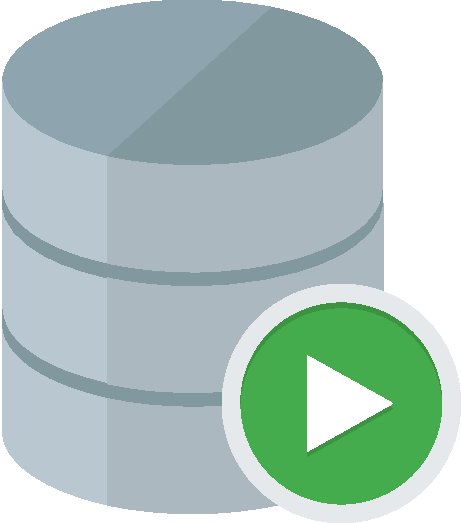
\includegraphics[height=8mm]{images/sec5/oraclesqldeveloper.pdf} \\\textbf{Oracle SQL}\\\textbf{Developer}
} & Vue \\
{
\includegraphics[height=7mm]{images/sec5/postman.pdf} \\\textbf{Postman}
} & Postman est un environnement de développement d'API complet permettant de concevoir, de mocker, de tester, de surveiller et de publier des API à partir de l'interface utilisateur Postman.\\
{
\includegraphics[height=7mm]{images/sec5/sonarcube.pdf} \\\textbf{SonarQube}
} & Vue \\
{
\includegraphics[width=7mm]{images/sec5/sourcetree.pdf} \\\textbf{Sourcetree}
} & Vue \\
{
\includegraphics[height=8mm]{images/sec5/wildfly.pdf} \\\textbf{WildFly}
} & Vue \\
{
\includegraphics[height=4.5mm]{images/sec5/zoom.pdf} \\\textbf{Zoom}
} & Vue \\
\end{longtblr}
\subsection{Outils utilisés pour la réalisation de ce rapport}
Adobe Illustrator
Draw.io
LaTeX
Figma
Vs code
\addcontentsline{toc}{subsection}{Conclusion}
\subsection*{Conclusion}
%%%%%%%%%%%%%%%%%%
